\section{Klassifizierung}
Statt die genaue Regenmenge vorherzusagen, stellten wir drei Kategorien auf: kein Regen ($= 0mm$), wenig Regen ($\leq 8mm$) und viel Regen ($> 8mm$). Diese Kategorien haben wir als One-Hot-Vector kodiert. `[1, 0, 0]` entspricht hierbei kein Regen, sodass man aus der ersten Dimension der Vorhersage einfach ein Vorschaubild generieren kann aus dem man gleich feststellen kann, ob es am jeweiligen Pixel regnet oder nicht.

Für das Training mit Kategorien kann man nicht mehr den MSE verwenden, hier würde selbst nach 80 Epochen nur \gqq{kein Regen} vorhergesagt. Stattdessen wurde als Loss-Funktion die \gqq{Categorical Crossentropy} von Keras verwendet; die binäre Crossentropy können wir nicht verwenden, weil wir mehr als zwei Kategorien verwenden. Die \gqq{Categorical Crossentropy} funktioniert relativ gut, aber es wird ein Blob vorhersagt, der etwas über den Bereich ragt, in dem es eigentlich regnet.

Danach wurde noch die Aktivierungsfunktion für den Output-Layer Sigmoid durch Softmax ersetzt. Dadurch erscheint das Vorschaubild etwas verwaschener, aber der Blob um das Regengebiet wird kleiner und die Differenz zum Referenzbild wird kleiner.

Wenn man die Aktivierungsfunktion der Hidden-Layer (von ReLu) zu Tanh verändert, verbessert sich auch die Kategorisierung: der Blob nähert sich weiter dem Regengebiet aus dem zu vorhersagendem Bild an, ist aber immer noch merkbar größer und franst an den kanten aus.

Als nächstes wird die Metrik \gqq{categorical\_accuracy} verwendet, um die Vorhersage zu überwachen. Dadurch kann der Fortschritt beim Trainieren besser überwacht werden.


\subsection{Training}
Für das Training wurden alle Daten der 18 Jahre verwendet, partitioniert in Trainings- und Evaluationsdaten. Als Lossfunktion wurde der MSE verwendet, der den Unterschied über alle Pixel kumuliert, weswegen so hohe Werte in den Abbildungen vorkommen (1100x900 Pixel). Da das Training auf der GPU weniger al 10~Sekunden pro Epoche dauert, wurden gleich 3072 Epochen trainiert.

In Abbildung~\ref{fig:lernkurven} sind die Lernkurven des Trainings nebeneinander dargestellt, links steht das Training des Netzes mit Softmax als Aktivierungsfunktion des Hidden Layer und rechts ist das selbe Netz mit TanH als Aktivierungsfunktion. Man sieht jedoch, dass es ab etwa 1500~Epochen (x-Achse) keine Verbesserungen mehr gibt.

\begin{figure}[ht]
\centering
\begin{subfigure}{0.5\textwidth}
\centering
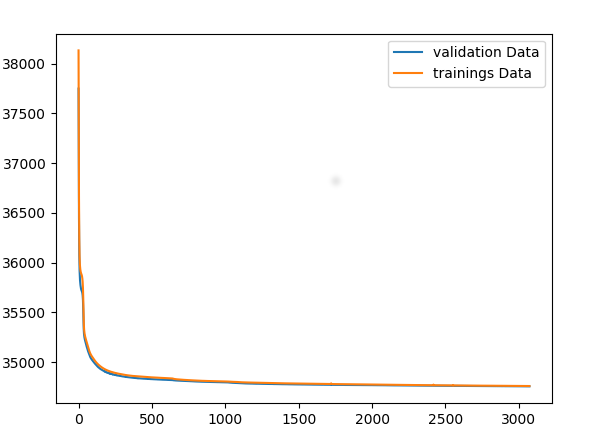
\includegraphics[width=\linewidth]{pics/lernkurve_activationHidden-softmax_activationOutput-softmax}
\caption{Lernkurve (Hidden layer: Softmax)}
\label{fig:lernkurveSoftmax}
\end{subfigure}%
\begin{subfigure}{0.5\textwidth}
\centering
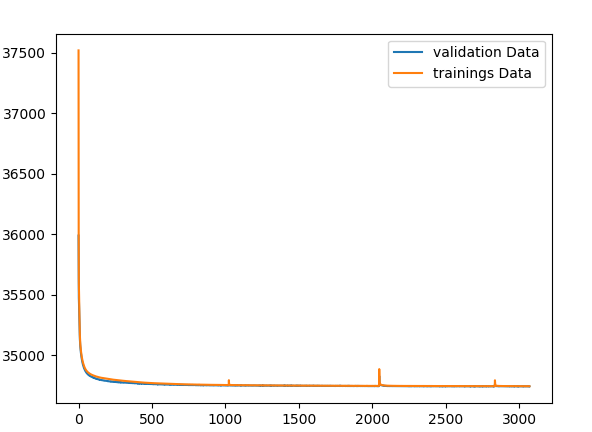
\includegraphics[width=\linewidth]{pics/lernkurve_activationHidden-tanh_activationOutput-softmax}
\caption{Lernkurve (Hidden layer: Tanh)}
\label{fig:lernkurveTanh}
\end{subfigure}%
\caption[Lernkurven verschiedener Aktivierungsfkt. der Hidden Layer]{Lernkurven von zwei verschiedenen Aktivierungsfunktionen der Hidden Layer. Ab etwa der tausendsten Epoche gibt es kaum noch eine Verbesserung.}
\label{fig:lernkurven}
\end{figure}



\subsection{Auswertung}
Zu den Netzen mit den verschiedenen Aktivierungsfunktionen wurden jeweils eine Confustion-Matrix erstellt (siehe Tabellen~\ref{tab:confusionSoftmax} und~\ref{tab:confusionTanh}). An beiden Matrizen kann man sehen, dass beide Aktivierungsfunktionen für einzelne Pixel statistisch ähnliche Ergebnisse liefern.

Bei beiden Matrizen ist gleich, dass, falls kein Regen vorhergesagt wird, in 96,1\% respektive 96,3\% auch tatsächlich kein Regen eintrifft. Wird wenig Regen vorhergesagt, ist die Unsicherheit recht groß: zu rund 20\% regnet es gar nicht oder zu etwa 16\% regnet es stark. Zu einem Fünftel kann es also sein, dass hier die Vorhersage \gqq{Regen} nicht eintrifft. Wird starker Regen vorausgesagt, trifft zu gut 68\% auch starker Regen ein, zu fast 26\% wenig Regen oder gut 5\% kein Regen. Hier trifft die Vorhersage \gqq{Regen} also zu 95\% ein.

\begin{table}[ht]
\centering
\begin{tabular}{lr|rrr}
    &                      & \multicolumn{3}{c}{Vorhersage}\\
    &                      & \textbf{Kein Regen} & \textbf{Wenig Regen} & \textbf{Viel Regen}\\\hline
\multirow{3}{*}{\rotatebox{90}{Daten}}
    & \textbf{Kein Regen}  & 2227245 (96,1\%)    & 33383 (19,9\%)       & 3762 (05,7\%)\\
    & \textbf{Wenig Regen} & 81116 (03,5\%)      & 106434 (63,4\%)      & 17077 (25,9\%)\\
    & \textbf{Viel Regen}  & 9695 (00,4\%)       & 27930 (16,7\%)       & 45166 (68,4\%)\\
\end{tabular}
\caption[Confustion-Matrix (Drei Kategorien, Hidden Layer: Softmax)]{Confustion-Matrix (Drei Kategorien, Aktivierungsfunktion der Hidden Layer: Softmax)}
\label{tab:confusionSoftmax}
\end{table}

\begin{table}[ht]
\centering
\begin{tabular}{lr|rrr}
    &                      & \multicolumn{3}{c}{Vorhersage}\\
    &                      & \textbf{Kein Regen} & \textbf{Wenig Regen} & \textbf{Viel Regen}\\\hline
\multirow{3}{*}{\rotatebox{90}{Daten}}
    & \textbf{Kein Regen}  & 2225229 (96,3\%)    & 35527 (20,4\%)       & 3634 (05,4\%)\\
    & \textbf{Wenig Regen} & 76988 (03,3\%)      & 110399 (63,5\%)      & 17240 (25,8\%)\\
    & \textbf{Viel Regen}  & 8849 (00,4\%)       & 27969 (16,1\%)       & 45973 (68,8\%)\\
\end{tabular}
\caption[Confustion-Matrix (Drei Kategorien, Hidden Layer: Tanh)]{Confustion-Matrix (Drei Kategorien, Aktivierungsfunktion Hidden Layer: Tanh)}
\label{tab:confusionTanh}
\end{table}

Bei der Vorhersage von zusammenhängenden Niederschlagsmengen auf einer Karte gibt es Unterschiede zwischen den Aktivierungsfunktionen der Hidden Layer, während es auf die Wahrscheinlichkeit der einzelnen Pixel kaum Unterschiede gab.
Das UNet mit TanH als Aktivierungsfunktion der Hidden Layer erzeugt größere (und leicht rundere) Blobs (Abbildung~\ref{fig:hiddenActivationTanh}). Bei Softmax werden schräge Kanten besser vorhergesagt (Abbildung~\ref{fig:hiddenActivationSoftmax}).
\begin{figure}[ht]
\centering
\begin{subfigure}{0.5\textwidth}
\centering
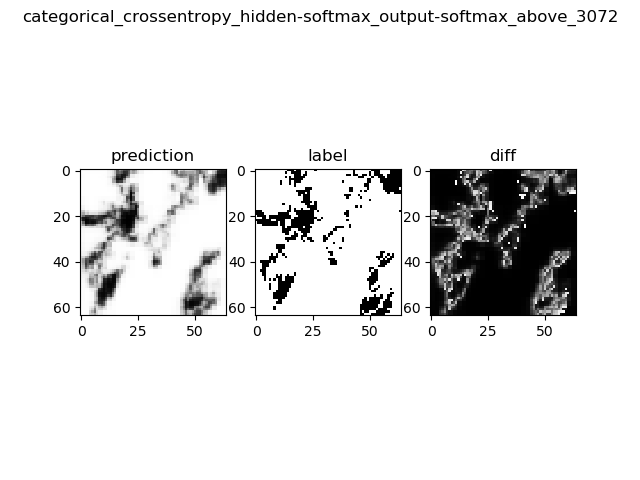
\includegraphics[width=\linewidth]{pics/categorical_crossentropy_hidden-softmax_output-softmax_above_3072}
\caption{Hidden layer activation: Softmax}
\label{fig:hiddenActivationSoftmax}
\end{subfigure}%
\begin{subfigure}{0.5\textwidth}
\centering
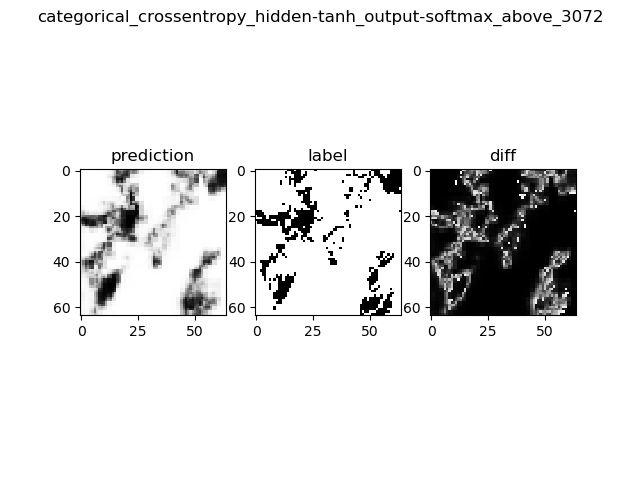
\includegraphics[width=\linewidth]{pics/categorical_crossentropy_hidden-tanh_output-softmax_above_3072}
\caption{Hidden layer activation: Tanh}
\label{fig:hiddenActivationTanh}
\end{subfigure}%
\caption[Vergleich von Aktivierungsfunktionen der Hidden-Layer]{Vergleich von Aktivierungsfunktionen der Hidden-Layer nach je 3072 Epochen. Aktivierungsfunktion der Output Layer ist jedes mal Softmax.}
\label{fig:activatinHidden}
\end{figure}


\subsubsection{Training mit zwei Kategorien}
Daraufhin versuchten wir die Vorhersage mit nur zwei Kategorien (Regen / Kein Regen) durchzuführen um festzustellen, ob die Vorhersage auf diese Weise besser funktioniert als die mit den drei bisherigen Kategorien. Dazu trainierten wir noch einmal das Netz mit zwei Kategorien und stellen die Confusion Matrix auf (siehe Tabelle~\ref{tab:confusionTwoCategoriesThresholdZero}). Bei einem Threshold von 0 erhält man fast gleiche Wahrscheinlichkeiten wie bei 3 Kategorien für Regen und Kein Regen: Falls kein Regen vorhergesagt wurde, regnet es zu 96\% nicht; und falls Regen vorhergesagt wurde regnet es zu gut 80\%.

\begin{table}[ht]
\centering
\begin{tabular}{lr|rr}
    &                      & \multicolumn{2}{c}{Vorhersage}\\
    &                      & \textbf{Kein Regen} & \textbf{Regen}\\\hline
\multirow{3}{*}{\rotatebox{90}{Daten}}
    & \textbf{Kein Regen}  & 2218754 (96,3\%)    & 45636 (18,4\%)\\
    & \textbf{Regen}       & 85427 (03,7\%)      & 201991 (81,6\%)\\
\end{tabular}
\caption{Confustion-Matrix (Zwei Kategorien, Threshold: 0, Softmax)}
\label{tab:confusionTwoCategoriesThresholdZero}
\end{table}

Verwendet man einen Threshold von 2 (mm) für die Generierung der Kategorien, verschlechtern sich die Wahrscheinlichkeiten leicht (siehe Tabelle~\ref{tab:confusionTwoCategoriesThresholdTwo}). Falls Regen vorhergesagt wurde, ist die Kein-Regen-Wahrscheinlichkeit nun 19,6\%, statt 18,4\%. Die Wahrscheinlichkeit von Regen, falls kein Regen vorhergesagt wurde, wird dafür minimal besser: 3,3\% statt 3,7\%.
\begin{table}[ht]
\centering
\begin{tabular}{lr|rr}
    &                      & \multicolumn{2}{c}{Vorhersage}\\
    &                      & \textbf{Kein Regen} & \textbf{Regen}\\\hline
\multirow{3}{*}{\rotatebox{90}{Daten}}
    & \textbf{Kein Regen}  & 2272947 (96,7\%)    & 39276 (19,6\%)\\
    & \textbf{Regen}       & 78475 (03,3\%)      & 161110 (80,4\%)\\
\end{tabular}
\caption{Confustion-Matrix (Zwei Kategorien, Threshold: 2, Softmax)}
\label{tab:confusionTwoCategoriesThresholdTwo}
\end{table}

Erhöht man den Threshold weiter auf 4, verdeutlicht sich der Trend aus der letzten Confusion Matrix (siehe Tabelle~\ref{tab:confusionTwoCategoriesThresholdFour}): die Wahrscheinlichkeit, dass für Regen \gqq{kein Regen} vorhergesagt wird, sinkt auf 2,7\%, die Wahrscheinlichkeit, dass Regen vorhergesagt wird und nicht eintrifft, steigt auf 23,2\%.
\begin{table}[ht]
\centering
\begin{tabular}{lr|rr}
    &                      & \multicolumn{2}{c}{Vorhersage}\\
    &                      & \textbf{Kein Regen} & \textbf{Regen}\\\hline
\multirow{3}{*}{\rotatebox{90}{Daten}}
    & \textbf{Kein Regen}  & 2376736 (97,3\%)    & 25441 (23,2\%)\\
    & \textbf{Regen}       & 65381 (02,7\%)      & 84250 (77,8\%)\\
\end{tabular}
\caption{Confustion-Matrix (Zwei Kategorien, Threshold: 4, Softmax)}
\label{tab:confusionTwoCategoriesThresholdFour}
\end{table}

Man sieht also, dass die Vorhersage ob Regen eintrifft oder nicht, bei drei Kategorien und zwei Kategorien (bei einem Threshold von 0) fast gleich ausfällt und  die Erhöhung des Thresholds die Genauigkeit senkt. Die genaue Regenmenge vorauszusagen hat sich als schwierig herausgestellt, aber man weiß zumindest (fast) sicher, dass man, wenn kein Regen vorhergesagt wird, nicht nass wird.

\subsection{ROC-Kurve bei zwei Kategorien}

Zur Überprüfung des Verhalten der Genauigkeit bei Anpassung des Treshold wird eine receiver operating characteristic-curve (ROC) verwendet. Siehe Abbildung \ref{roc}. Diese dient zum Vergleich der Confusion Matrizen mit verschiedenen Tresholds und damit der Performance des Netzes. \newline

Auf der X-Achse wird die True Positive Rate (Sensitivität) abgebildet. Diese beschreibt die Rate der richtig kategorisierten positiven Ereignisse (In unserem Fall: Kein Regen vorhergesagt und es regnet tatsächlich nicht). \newline

\begin{align*}
  TPR \quad	 {=} \quad True Positives \quad / \quad(True Positive + False Negatives)
\end{align*}

Auf der Y-Achse wird die False Positive Rate abgebildet. Diese beschreibt die Rate der falsch kategorisierten negativen Ereignisse (In unserem Fall: Kein Regen vorhergesagt aber es regnet tatsächlich) und der Gesamtanzahl der negativen Ereignisse. \newline

\begin{align*}
  FPR \quad	 {=} \quad False Positives \quad / \quad(False Positive + True Negatives)
\end{align*}

In einem Optimalen Szenario wäre der Wert der TPR gleich eins und der Wert der FPR gleich Null. 


\begin{figure}[H]
	\centering
	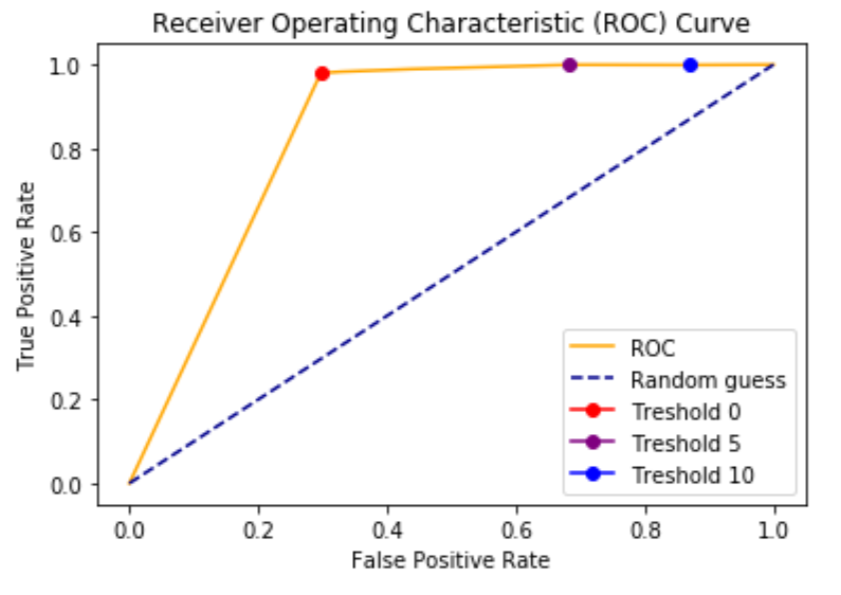
\includegraphics[width=0.6\textwidth]{pics/roc.PNG}
	\caption{ROC curve}
	\label{roc}
\end{figure}

\subsubsection{Interpretation ROC}
Wie bereits vermutet, verschlechtert sich die Genauigkeit mit einer Erhöhung eines Tresholds, der mit Null daher den bestmöglichen Wert hat.
Außerdem kann dadurch nachgewiesen werden, dass die Genauigkeit höher als beim zufälligen Auswählen ist.

\subsection{Herausforderungen in diesem Kapitel}
In diesem Kapitel gab es zwei große Herausforderungen: zum einen war es schwierig die richtigen Kategorien zu finden, und zum anderen musste sich herausstellen, wie sich die verschiedenen Aktivierungsfunktionen auswirken.

Die drei Kategorien haben sich als nicht ganz optimal herausgestellt, denn mit zwei Kategorien können wir aussagekräftigere Angaben geben: wir können sicherer angeben ob es regnet oder nicht.

Die Aktivierungsfunktionen haben sich nur auf die Form der Blobs der Niederschlagsmengen ausgewirkt (Abbildung~\ref{fig:activatinHidden}), aber weniger auf die Regen-Wahrscheinlichkeit der einzelnen Punkte (siehe Tabellen~\ref{tab:confusionSoftmax} und \ref{tab:confusionTanh}).
